\documentclass{standalone}
\usepackage{tikz}
\usetikzlibrary{patterns, positioning}


\begin{document}
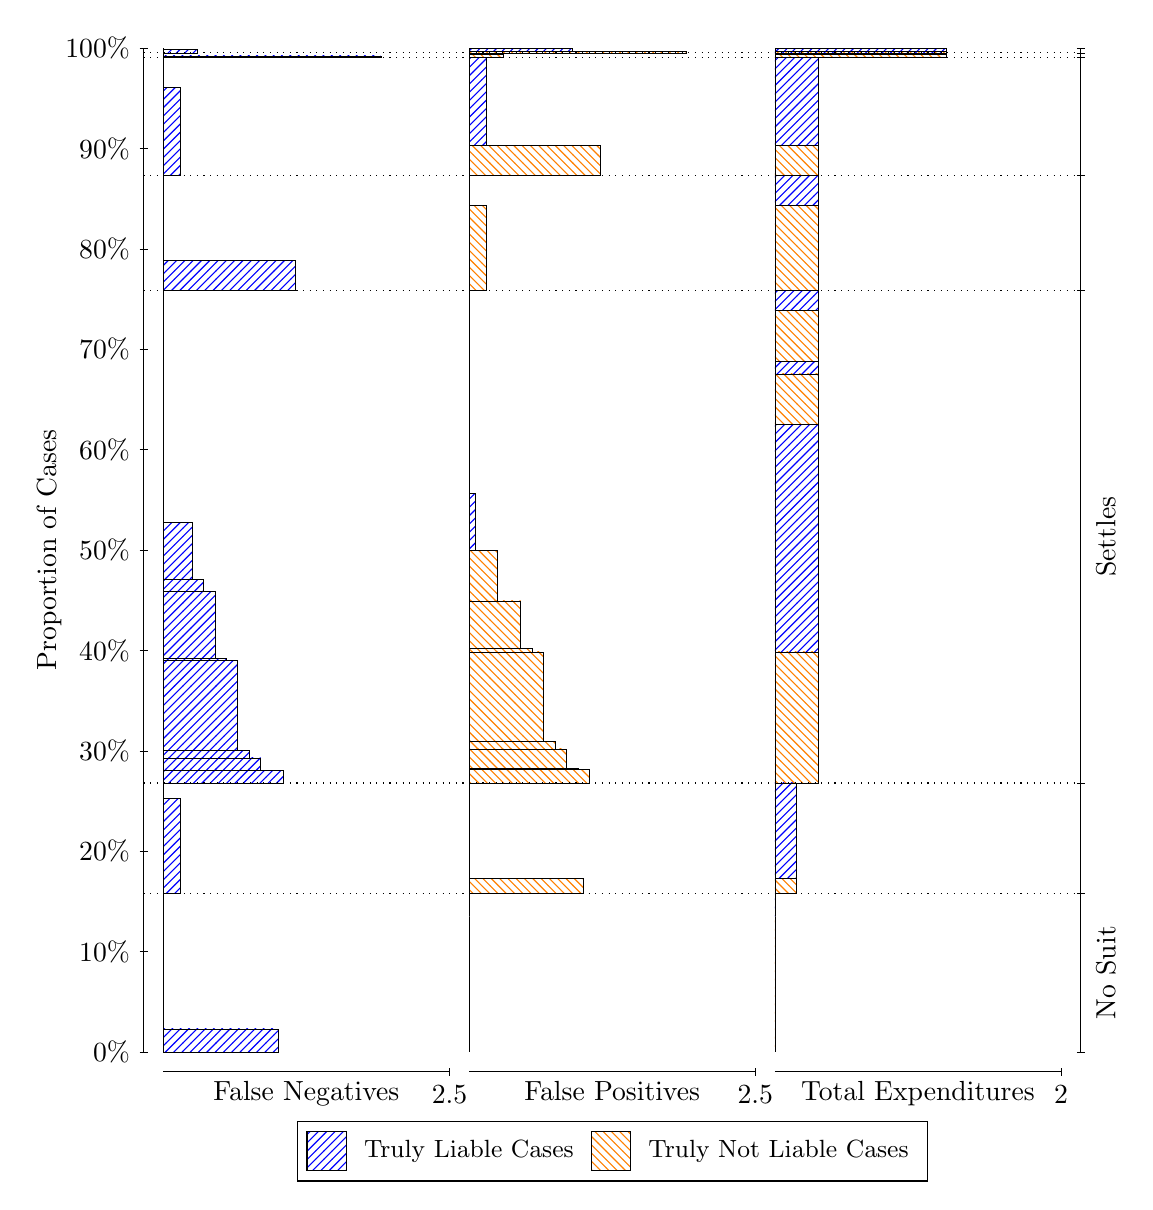
\begin{tikzpicture}
\draw[black, very thin] (1.5,1.75) -- (1.5,14.5);
\node[rotate=90, text=black, anchor=center] at (0.3, 8.125) {Proportion of Cases};
\draw[black, very thin] (1.45,1.75) -- (1.55,1.75);
\node[text=black, anchor=east] at (1.45, 1.75) {0\%};
\draw[black, very thin] (1.45,3.025) -- (1.55,3.025);
\node[text=black, anchor=east] at (1.45, 3.025) {10\%};
\draw[black, very thin] (1.45,4.3) -- (1.55,4.3);
\node[text=black, anchor=east] at (1.45, 4.3) {20\%};
\draw[black, very thin] (1.45,5.575) -- (1.55,5.575);
\node[text=black, anchor=east] at (1.45, 5.575) {30\%};
\draw[black, very thin] (1.45,6.85) -- (1.55,6.85);
\node[text=black, anchor=east] at (1.45, 6.85) {40\%};
\draw[black, very thin] (1.45,8.125) -- (1.55,8.125);
\node[text=black, anchor=east] at (1.45, 8.125) {50\%};
\draw[black, very thin] (1.45,9.4) -- (1.55,9.4);
\node[text=black, anchor=east] at (1.45, 9.4) {60\%};
\draw[black, very thin] (1.45,10.675) -- (1.55,10.675);
\node[text=black, anchor=east] at (1.45, 10.675) {70\%};
\draw[black, very thin] (1.45,11.95) -- (1.55,11.95);
\node[text=black, anchor=east] at (1.45, 11.95) {80\%};
\draw[black, very thin] (1.45,13.225) -- (1.55,13.225);
\node[text=black, anchor=east] at (1.45, 13.225) {90\%};
\draw[black, very thin] (1.45,14.5) -- (1.55,14.5);
\node[text=black, anchor=east] at (1.45, 14.5) {100\%};

\draw[black, very thin] (13.4,1.75) -- (13.4,14.5);
\draw[black, very thin] (13.35,1.75) -- (13.45,1.75);
\node[anchor=west] at (13.35, 1.75) {};
\draw[black, very thin] (13.35,3.7628) -- (13.45,3.7628);
\node[anchor=west] at (13.35, 3.7628) {};
\draw[black, very thin] (13.35,5.1664) -- (13.45,5.1664);
\node[anchor=west] at (13.35, 5.1664) {};
\draw[black, very thin] (13.35,11.422) -- (13.45,11.422);
\node[anchor=west] at (13.35, 11.422) {};
\draw[black, very thin] (13.35,12.882) -- (13.45,12.882);
\node[anchor=west] at (13.35, 12.882) {};
\draw[black, very thin] (13.35,14.382) -- (13.45,14.382);
\node[anchor=west] at (13.35, 14.382) {};
\draw[black, very thin] (13.35,14.439) -- (13.45,14.439);
\node[anchor=west] at (13.35, 14.439) {};
\draw[black, very thin] (13.35,14.5) -- (13.45,14.5);
\node[anchor=west] at (13.35, 14.5) {};

\draw[black, very thin, pattern color=blue, pattern=north east lines] (1.75,1.75) rectangle (3.2033,2.0443);
\draw[black, very thin, pattern color=orange, pattern=north west lines] (1.75,2.0443) rectangle (1.75,3.7628);
\draw[black, very thin, pattern color=blue, pattern=north east lines] (1.75,3.7628) rectangle (1.968,4.9701);
\draw[black, very thin, pattern color=orange, pattern=north west lines] (1.75,4.9701) rectangle (1.75,5.1664);
\draw[black, very thin, pattern color=blue, pattern=north east lines] (1.75,5.1664) rectangle (3.276,5.3227);
\draw[black, very thin, pattern color=blue, pattern=north east lines] (1.75,5.3227) rectangle (2.9853,5.4845);
\draw[black, very thin, pattern color=blue, pattern=north east lines] (1.75,5.4845) rectangle (2.84,5.5803);
\draw[black, very thin, pattern color=blue, pattern=north east lines] (1.75,5.5803) rectangle (2.6947,6.7202);
\draw[black, very thin, pattern color=blue, pattern=north east lines] (1.75,6.7202) rectangle (2.5493,6.7523);
\draw[black, very thin, pattern color=blue, pattern=north east lines] (1.75,6.7523) rectangle (2.404,7.5955);
\draw[black, very thin, pattern color=blue, pattern=north east lines] (1.75,7.5955) rectangle (2.2587,7.7472);
\draw[black, very thin, pattern color=blue, pattern=north east lines] (1.75,7.7472) rectangle (2.1133,8.4724);
\draw[black, very thin, pattern color=orange, pattern=north west lines] (1.75,8.4724) rectangle (1.75,11.422);
\draw[black, very thin, pattern color=blue, pattern=north east lines] (1.75,11.422) rectangle (3.4213,11.805);
\draw[black, very thin, pattern color=orange, pattern=north west lines] (1.75,11.805) rectangle (1.75,12.882);
\draw[black, very thin, pattern color=blue, pattern=north east lines] (1.75,12.882) rectangle (1.968,14.005);
\draw[black, very thin, pattern color=orange, pattern=north west lines] (1.75,14.005) rectangle (1.75,14.382);
\draw[black, very thin, pattern color=blue, pattern=north east lines] (1.75,14.382) rectangle (4.5113,14.4);
\draw[black, very thin, pattern color=orange, pattern=north west lines] (1.75,14.4) rectangle (1.75,14.439);
\draw[black, very thin, pattern color=blue, pattern=north east lines] (1.75,14.439) rectangle (2.186,14.482);
\draw[black, very thin, pattern color=orange, pattern=north west lines] (1.75,14.482) rectangle (1.75,14.5);
\draw[black, very thin, pattern color=orange, pattern=north west lines] (5.6333,1.75) rectangle (5.6333,3.4686);
\draw[black, very thin, pattern color=blue, pattern=north east lines] (5.6333,3.4686) rectangle (5.6333,3.7628);
\draw[black, very thin, pattern color=orange, pattern=north west lines] (5.6333,3.7628) rectangle (7.0867,3.9591);
\draw[black, very thin, pattern color=blue, pattern=north east lines] (5.6333,3.9591) rectangle (5.6333,5.1664);
\draw[black, very thin, pattern color=orange, pattern=north west lines] (5.6333,5.1664) rectangle (7.1593,5.3355);
\draw[black, very thin, pattern color=orange, pattern=north west lines] (5.6333,5.3355) rectangle (7.014,5.3562);
\draw[black, very thin, pattern color=orange, pattern=north west lines] (5.6333,5.3562) rectangle (6.8687,5.5995);
\draw[black, very thin, pattern color=orange, pattern=north west lines] (5.6333,5.5995) rectangle (6.7233,5.6931);
\draw[black, very thin, pattern color=orange, pattern=north west lines] (5.6333,5.6931) rectangle (6.578,6.8316);
\draw[black, very thin, pattern color=orange, pattern=north west lines] (5.6333,6.8316) rectangle (6.4327,6.874);
\draw[black, very thin, pattern color=orange, pattern=north west lines] (5.6333,6.874) rectangle (6.2873,7.4789);
\draw[black, very thin, pattern color=orange, pattern=north west lines] (5.6333,7.4789) rectangle (5.9967,8.1158);
\draw[black, very thin, pattern color=blue, pattern=north east lines] (5.6333,8.1158) rectangle (5.706,8.8411);
\draw[black, very thin, pattern color=blue, pattern=north east lines] (5.6333,8.8411) rectangle (5.6333,11.422);
\draw[black, very thin, pattern color=orange, pattern=north west lines] (5.6333,11.422) rectangle (5.8513,12.498);
\draw[black, very thin, pattern color=blue, pattern=north east lines] (5.6333,12.498) rectangle (5.6333,12.882);
\draw[black, very thin, pattern color=orange, pattern=north west lines] (5.6333,12.882) rectangle (7.3047,13.259);
\draw[black, very thin, pattern color=blue, pattern=north east lines] (5.6333,13.259) rectangle (5.8513,14.382);
\draw[black, very thin, pattern color=orange, pattern=north west lines] (5.6333,14.382) rectangle (6.0693,14.421);
\draw[black, very thin, pattern color=blue, pattern=north east lines] (5.6333,14.421) rectangle (5.6333,14.439);
\draw[black, very thin, pattern color=orange, pattern=north west lines] (5.6333,14.439) rectangle (8.3947,14.457);
\draw[black, very thin, pattern color=blue, pattern=north east lines] (5.6333,14.457) rectangle (6.9413,14.5);
\draw[black, very thin, pattern color=orange, pattern=north west lines] (9.5167,1.75) rectangle (9.5167,3.4686);
\draw[black, very thin, pattern color=blue, pattern=north east lines] (9.5167,3.4686) rectangle (9.5167,3.7628);
\draw[black, very thin, pattern color=orange, pattern=north west lines] (9.5167,3.7628) rectangle (9.7892,3.9591);
\draw[black, very thin, pattern color=blue, pattern=north east lines] (9.5167,3.9591) rectangle (9.7892,5.1664);
\draw[black, very thin, pattern color=orange, pattern=north west lines] (9.5167,5.1664) rectangle (10.062,6.8316);
\draw[black, very thin, pattern color=blue, pattern=north east lines] (9.5167,6.8316) rectangle (10.062,9.7237);
\draw[black, very thin, pattern color=orange, pattern=north west lines] (9.5167,9.7237) rectangle (10.062,10.361);
\draw[black, very thin, pattern color=blue, pattern=north east lines] (9.5167,10.361) rectangle (10.062,10.517);
\draw[black, very thin, pattern color=orange, pattern=north west lines] (9.5167,10.517) rectangle (10.062,11.164);
\draw[black, very thin, pattern color=blue, pattern=north east lines] (9.5167,11.164) rectangle (10.062,11.422);
\draw[black, very thin, pattern color=orange, pattern=north west lines] (9.5167,11.422) rectangle (10.062,12.498);
\draw[black, very thin, pattern color=blue, pattern=north east lines] (9.5167,12.498) rectangle (10.062,12.882);
\draw[black, very thin, pattern color=orange, pattern=north west lines] (9.5167,12.882) rectangle (10.062,13.259);
\draw[black, very thin, pattern color=blue, pattern=north east lines] (9.5167,13.259) rectangle (10.062,14.382);
\draw[black, very thin, pattern color=orange, pattern=north west lines] (9.5167,14.382) rectangle (11.697,14.421);
\draw[black, very thin, pattern color=blue, pattern=north east lines] (9.5167,14.421) rectangle (11.697,14.439);
\draw[black, very thin, pattern color=orange, pattern=north west lines] (9.5167,14.439) rectangle (11.697,14.457);
\draw[black, very thin, pattern color=blue, pattern=north east lines] (9.5167,14.457) rectangle (11.697,14.5);
\draw[black, dotted] (1.5,3.7628) -- (13.4,3.7628);
\draw[black, dotted] (1.5,5.1664) -- (13.4,5.1664);
\draw[black, dotted] (1.5,11.422) -- (13.4,11.422);
\draw[black, dotted] (1.5,12.882) -- (13.4,12.882);
\draw[black, dotted] (1.5,14.382) -- (13.4,14.382);
\draw[black, dotted] (1.5,14.439) -- (13.4,14.439);
\draw[black, very thin] (1.75,1.5) -- (5.3833,1.5);
\node[text=black, anchor=north] at (3.5667, 1.5) {False Negatives};
\draw[black, very thin] (5.3833,1.45) -- (5.3833,1.55);
\node[text=black, anchor=north] at (5.3833, 1.45) {2.5};

\draw[black, very thin] (5.6333,1.5) -- (9.2667,1.5);
\node[text=black, anchor=north] at (7.45, 1.5) {False Positives};
\draw[black, very thin] (9.2667,1.45) -- (9.2667,1.55);
\node[text=black, anchor=north] at (9.2667, 1.45) {2.5};

\draw[black, very thin] (9.5167,1.5) -- (13.15,1.5);
\node[text=black, anchor=north] at (11.333, 1.5) {Total Expenditures};
\draw[black, very thin] (13.15,1.45) -- (13.15,1.55);
\node[text=black, anchor=north] at (13.15, 1.45) {2};

\node[text=black, centered, rotate=90] at (13.72, 2.7564) {No Suit};

\node[text=black, centered, rotate=90] at (13.72, 8.2941) {Settles};





\draw (7.449999999999999,1.5) node[draw=none] (baseCoordinate) {};
\begin{scope}[align=center]
        \matrix[scale=0.5, draw=black, below=0.5cm of baseCoordinate, nodes={draw}, column sep=0.1cm]{
            \node[rectangle, draw, minimum width=0.5cm, minimum height=0.5cm, pattern color=blue, pattern=north east lines] {}; &
            \node[draw=none, font=\small, text=black] (B) {Truly Liable Cases}; &
            \node[rectangle, draw, minimum width=0.5cm, minimum height=0.5cm, pattern color=orange, pattern=north west lines] {}; &
            \node[draw=none, font=\small, text=black] (B) {Truly Not Liable Cases}; \\
            };
\end{scope}

\end{tikzpicture}
\end{document}